\documentclass[twocolumn,10pt]{article}

\usepackage[a4paper,hmargin=1.5cm,vmargin=2.5cm,]{geometry}
\setlength{\columnsep}{0.7cm}
\usepackage{palatino}
\usepackage{graphicx}
\usepackage[utf8]{inputenc}
\usepackage{hyperref}
\usepackage{minted}
\usepackage{balance}
\usepackage{dblfloatfix}  
\usemintedstyle{colorful}
\usepackage[font=small,labelfont=bf]{caption}
\urlstyle{same} % no tt font for URLs
\newcommand{\blockade}{\rule{3em}{0.7em}}  %% Marker for things to change before submission
\newcommand{\fixme}[1]{[ \blockade FIXME: #1]}

\usepackage{natbib}
\bibliographystyle{genome_research}
\setcitestyle{aysep={}} 

\usepackage[dvipsnames]{xcolor}
\hypersetup{
    colorlinks,
    linkcolor={blue!50!black},
    citecolor={blue!50!black},
    urlcolor={blue!50!black}
}
\renewcommand{\dbltopfraction}{0.7}
\renewcommand{\textfraction}{0.2}

\begin{document}

\setcounter{secnumdepth}{0}


\twocolumn[{%
\centering
\textbf{\Large R/LinkedCharts: A novel approach for simple but powerful interactive data analysis}
\vspace{1.5ex}

Svetlana Ovchinnikova and Simon Anders\\
{\footnotesize Center for Molecular Biology of the University of Heidelberg, Germany}
\vspace{1.5ex}

24 January 2020
\vspace{6ex}
}]

\section{Abstract}
In any research project involving data-rich assays, exploratory data analysis is a crucial step. Typically,this involves jumping back and forth between visualizations that provide overview of the whole data and others that dive into details. In data quality assessment, for example, it might be very helpful to have one chart showing a summary statistic for all samples, and clicking on one of the data points would display details on this sample in a second plot. Setting up such interactively linked charts is usually too cumbersome and time-consuming to use them in \emph{ad hoc} analysis. We present R/LinkedCharts, a framework  that renders this tasks radically simple: Producing linked charts is as quickly done as is producing conventional static plots in R, requiring a data scientist to write only very few lines of simple R code to obtain complex and general visualization. We expect that the convenience of our new tool will enable data scientists and bioinformaticians to perform much deeper and more thorough EDA with much less effort. Furthermore, R/LinkedCharts apps, typically first written as quick-and-dirty hacks, can also later be polished to provide interactive data access in publication quality, thus contributing to open science.

\section{Introduction}

Effective data visualization has been crucial for scientific success since the first quantitative experiments. The continuously growing amount and complexity of available data over the last decades made the task more and more challenging. For a while, the only possible way to tackle the problem was to develop more elaborate types of plots employing colour, shape, transparency, and other visual aspects to combine multiple layers of information \citep{bertin_2011, tufte_1983, }. Yet, there are certain limits to how much information one can learn from a static image \citep{hegarty_2011}. Excessive details and multiple overlapping layers make it harder to grasp the crux of a plot. Thus, a researcher has to decide what information to keep and what to dismiss to convey the message better \citep{odonoghue_2018}. This is, arguably, an essential step since data often contain much noise and information irrelevant to the point one tries to make. Yet, it may be useful to provide the reader with a way to estimate the relevance of the omitted pieces of data on his or her own to avoid biases \citep{bresciani_2009} and thus boost confidence in reported data patterns.

With the advance of modern computer technology, interactive visualization emerged to offer new ways of presenting information, starting already in the 1970s \citep{newman_1979, becker_1987}. In an interactive figure, there is no need to fix all the parameters or to exclude any data that do not contribute to the main idea. Instead, the user gets a chance to experiment with data and details quickly and intuitively, concentrating at once on the plot's most exciting or suspicious parts. Numerous tools \citep{caldarola_2017} now provide means of inspecting many specific types of data with interactive tools, for example, in biology, metabolic maps \citep{noronha_2017}, geonome assemblies \citep{wick_2015}, scRNA-Seq data \citep{hillje_2020}, QTL data \citep{broman_2015} -- too name just a few examples. Besides such solution for very specific types of data, there are a number of general low-level frameworks to create interactive apps, such as D3 \citep{bostock_2011} and Vega-Lite \citep{satyanarayan_2015}, and more high-level but still general-purpose packages, including Vega \citep{satyanarayan_2016}, Shiny \citep{shiny}, BPG \citep{p_2019}, and plotly \citep{sievert_2019, sievert_2020}. However, the gap between these developmental frameworks and specialized apps is still wide, as we discuss below.

The advantage of interactivity lies beyond just simplifying navigation through big or complex data. When it merely takes a click or two to add changes to a plot, this urges a researcher not to put aside ideas or concerns and thus go through the data more thoroughly. At the same time, readers can check conclusions and claims of a paper on the fly, without going through all the script and analysis, thus making the findings more credible. Therefore, we believe that further integration of interactive tools in a researchers' routine can significantly improve the quality of studies \citep{shander_2016, yuk_2014}.

In practice, however, interactivity is still seriously underused during data analysis. Even though many authors now accompany their papers with an interactive resource to present their data and results (for example \citet{travaglini_2020, roider_2020, kalucka_2020}), these chiefly serve to present and communicate research that has already been completed. Commonly, it is only after most of the work on a project has been finished and the paper is being written up that researches spend a couple of days implementing a nice-looking interactive app to share their data and results with the scientific community \citep{batch_2017} to be added as supplement to their publication. 

\begin{figure*}[b]
	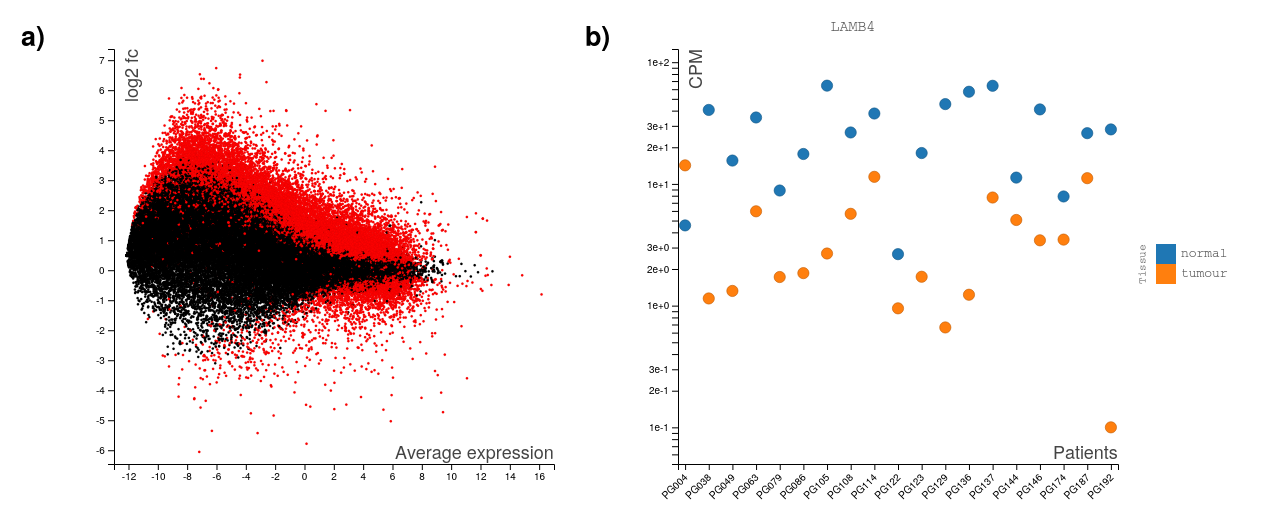
\includegraphics[width=\textwidth]{FigD/figD.png}
	\caption{An overview of genes differentially expressed in cancerous and normal tissues from \citet{conway_2015}. The MA plot (A) shows all the sequenced genes with their average expression on the X-axis and log-fold change on the Y-axis. Red indicates genes where the difference was reported as significant by the ``limma''  \citep{ritchie_2015}  package. The plot to the left (B) shows expression values (CPMs) for a selected gene (in this case, LAMB4) and all the patients. This figure is based on a LinkedCharts app, and its live version is provided in the supplement. When the user clicks on any point of the MA plot, the expression plot changes, showing the new selected gene. In this way, one can check immediately whether the genes labelled as significantly different are interesting for further study.}  
	\label{FigD}
\end{figure*}

Thus, visualization frameworks must be simple, to encourage practitioners to use interactivity as soon as there is merely the smallest hint that it might be useful. If frameworks for interactive visualization are too complicated, one will prefer to do most of the analysis by more conventional static means, and wait for a special occasion when it is worthwhile to invest time and effort into an interactive app. Furthermore, a good framework should be similar in design to common static visualization frameworks since tools with too specific interface tend to only be used by people with more extensive programming skill. Even if a researcher with less expertise in coding has an eager-to-help colleague, he or she may be unwilling to ask for assistance in petty everyday tasks and wait for something big.

Still, an attempt to simplify a tool may end in hard-coding and presetting too many parameters. As a result, a simple-to-use tool can require a particular data structure and be fit only for precisely matching data flow patterns. Any attempt of going beyond in-built limitations, if at all possible, can cost considerable effort. While much of routine work in the lab may involve only standardized steps and data types, intersting research tends to go beyond routine. Then, we need to avoid forcing a research problem into a predefined mould. Therefore, a sufficient degree of flexibility is required.

With the LinkedCharts framework, we tried to find a balance between the simplicity of usage and possibilities for customisation to make it suitable for interactive data exploration. It requires only basic coding skills to produce fully functional apps for \emph{ad hoc} analysis with just a few lines of code. With a little more effort, one can make a nicer looking app and customise the most commonly used plot settings (such as colours, labels, axes, etc.). Furthermore, by invetsi8ng a bit more effort, one can use LinkedCharts to make a "publication quality" app for deployment on a public server. Since the library is JavaScript-based, it can be combined with various existing web solutions. One can also write custom scripts that will change even hardcoded aspects of the library without making changes to the source code, rendering LinkedCharts extremely flexible. 

LinkedCharts is not fixed on any specific task. It is a toolbox, and its building blocks can be combined in any manner, the same way as one combines plots for a complex paper figure. All blocks share the same interface and very similar interactivity capabilities, which means that understanding one of them is enough to grasp the entire concept of LinkedCharts.

With all these, we hope that LinkedCharts can become a valuable asset for the scientific community that can be used both for everyday routine and for presenting one's research to a greater audience. LinkedCharts available as an R package (``rlc'', can be downloaded from CRAN) and as a JavaScript library. This paper's focus is on the R implementation of LinkedCharts, which we also refer to as R/LinkedCharts. 

\section{Results}

\subsection{Linking charts}

\begin{figure*}[t]
	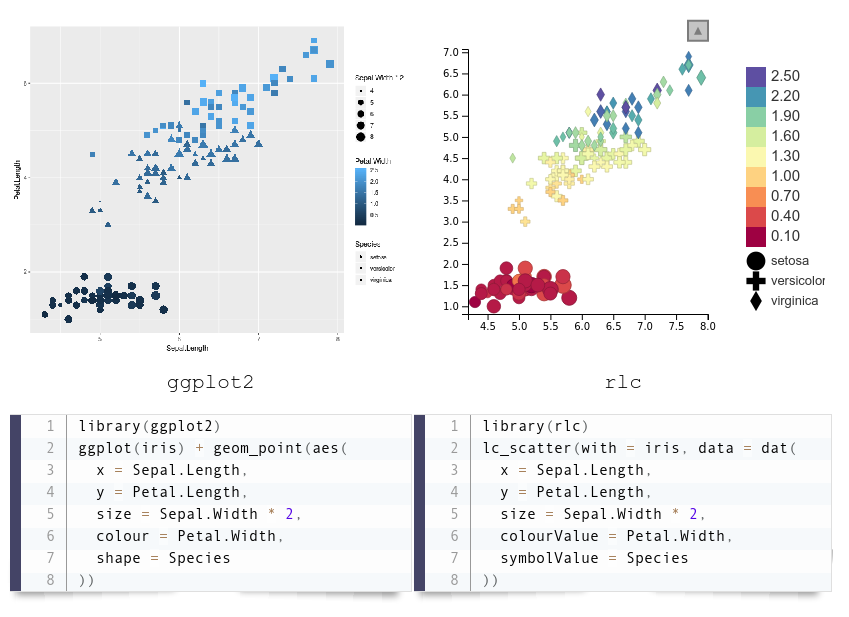
\includegraphics[width=\textwidth]{FigB/figB.png}
	\caption{Typical syntax of an R/LinkedCharts plot with comparison to the ``ggplot2'' \citep{wickham_2016} package, one of the most commonly used plotting libraries. Lines of the code are arranged to put the same aspects of the charts next to each other. ``iris'' dataset, which is one of the R built-in datasets, was used for this example. Both pieces of code are fully functional, and their output is shown above the code.}
	\label{FigB}
\end{figure*}

The central concept behind LinkedCharts is, as follows from the name, linking and focusing \citep{buja_1991}. We connect two or more plots so that manipulations with one of them affect the others. We now explain this concept using a simple example based on data from \citet{conway_2015}.

In that study, three samples were taken from each of 17 patients with oral cancer: of normal, cancerous, and dysplasia tissue. mRNA from all these samples was sequenced to obtain gene expression values. The standard question to ask based on these data is about differential expression between tissue types. Several packages offer functionality to answer such questions  \citep{ritchie_2015, love_2014}. Here, we have used the function \mintinline{R}{voom} from the ``limma'' package to compare normal and cancerous tissues. It is common to visualise such a comparison with an MA plot \citep{dudoit_2002}, where each dot represents a gene, showing the gene's average expression on the X-axis and log fold change between the two groups on the Y-axis (Fig \ref{FigD}(A)). Red dots correspond to genes that are considered significantly different between the two conditions (adjusted p-value $<$ 0.1). However, how does the difference in expression look like for every single patient? Is it consistent across all the patients or only detected in some of them? Are there any artifacts or outliers that cause the p-value to be too small?

To answer such questions, we can add another plot that shows expression values (as "counts per million", CPM) for all the individual samples (Fig \ref{FigD}(B)). This second plot can show expression for only one selected gene at a time, but LinkedCharts allows one to link it to the MA plot. Now, any mouse click on a point in the MA plot causes the plot to the right to display the individual expression values of the selected gene. Fig \ref{FigD} is based on the LinkedCharts app, which is provided in this paper's online supplement. We encourage the reader to pause for a moment and try it out. In the supplement, we also provide full code to generate the app and links to necessary data files to immediately get this app in one's R session and experiment with it. For this and all further examples, we provide two versions of code: minimal with only essential parameters needed to make the app functional, and more extended with custom colours, labels, etc. In the paper, we only focus on the minimal code.

To  explain the linking mechanism, we briefly discuss the code that generates the app from Fig \ref{FigD}. This is a minimal, but complete code for the app, suitable to illustrate the design principles of R/LinekdCharts. For now, we concentrate only on the highlighted lines.

\begin{figure*}[b]
	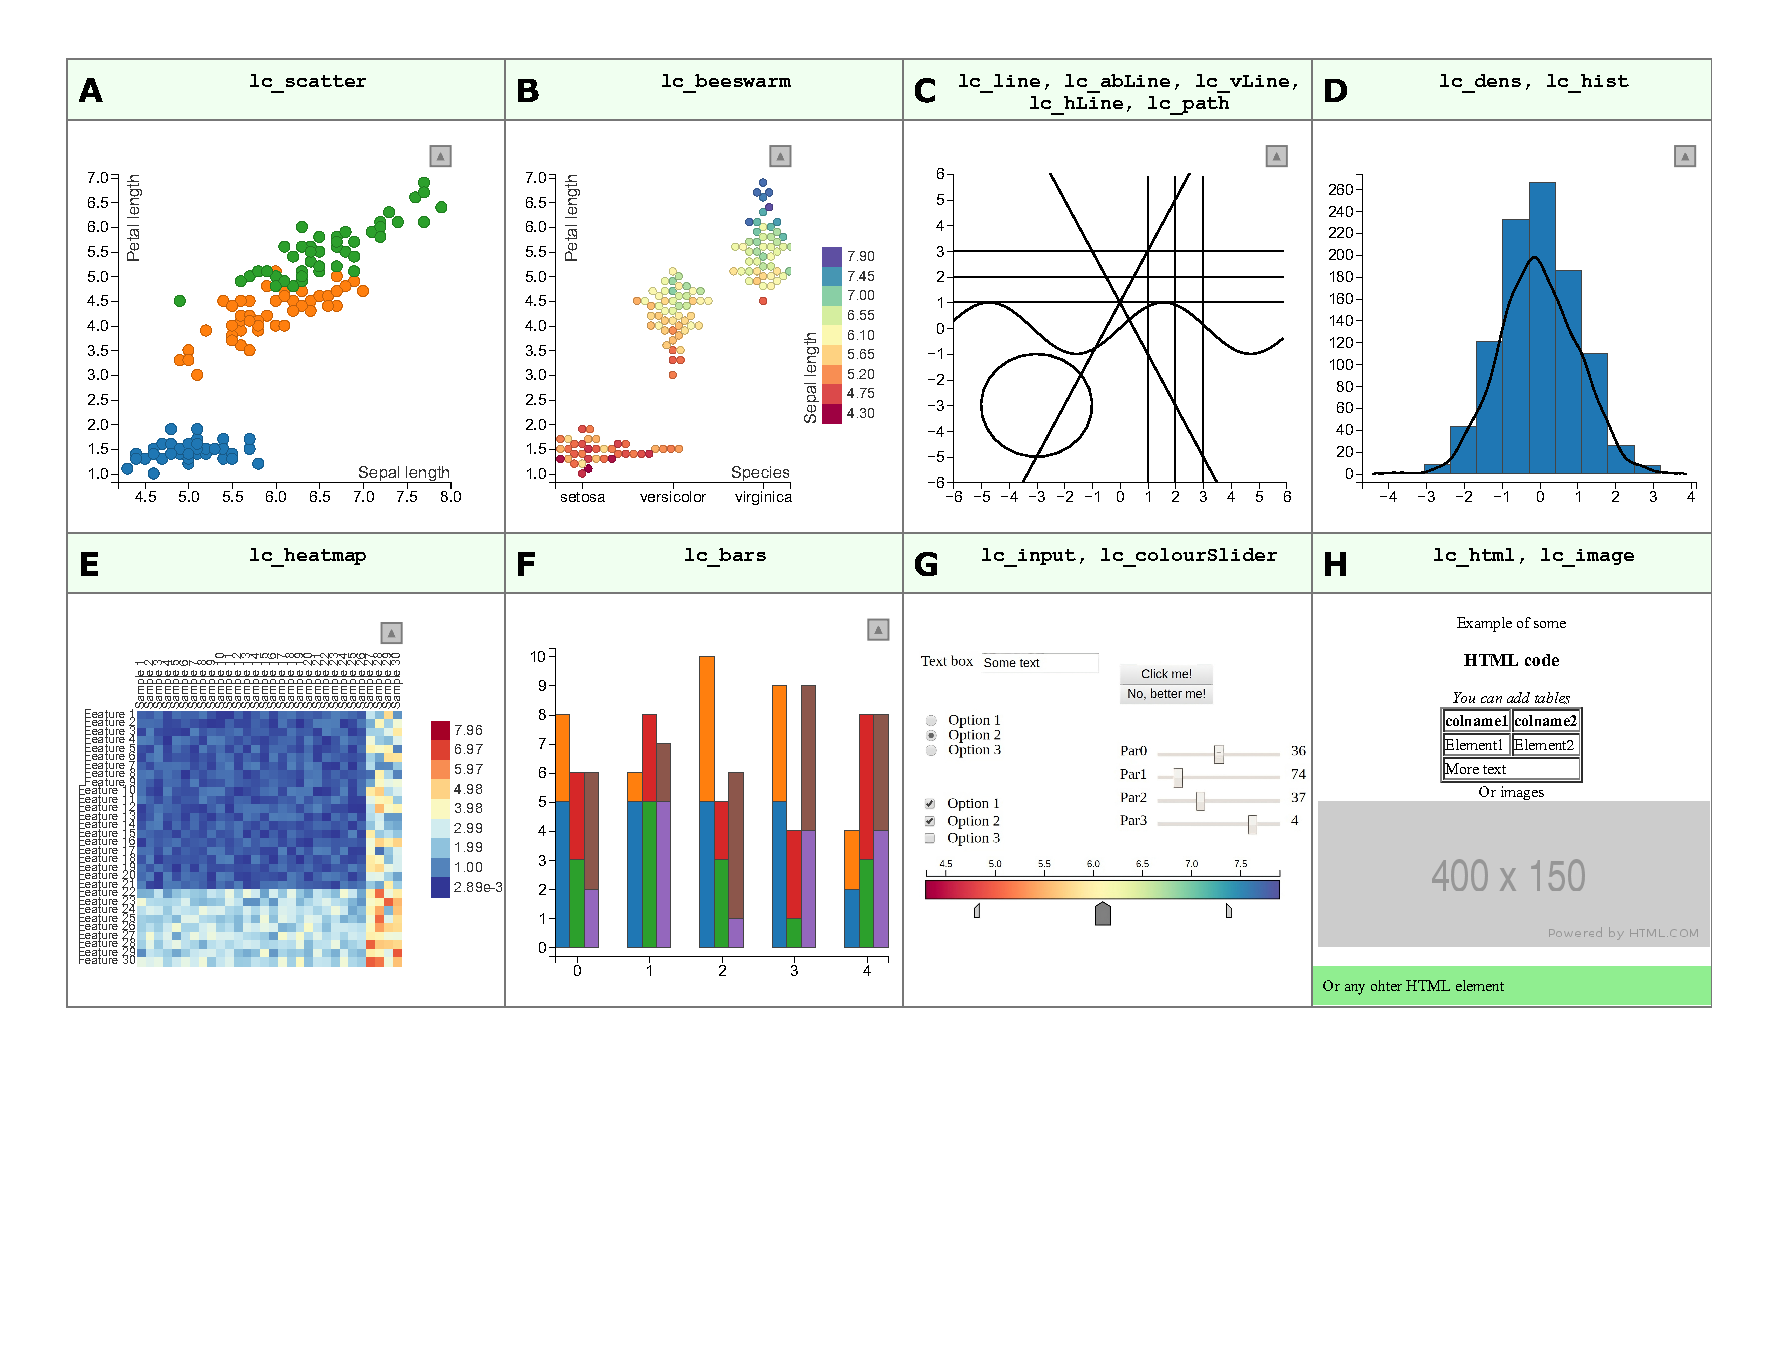
\includegraphics[width=\textwidth]{FigA/figA.png}
	\caption{Gallery of all available plotting functions in the ``rlc'' package. A scatter plot (A); a bee swarm plot (based on d3-beeswarm plugin \citep{lebeau_2017}) (B); a collection of various lines (C); a histogram and a density plot (density was multiplied by a factor of 500 to be visible on the same plot as the histogram) (D); a heatmap (E); a bar chart (F); a collection of interactive elements to gather input from the user (G); functions to add custom HTML code and static plots to the page (H). All these examples with code to create them can be found in the supplement.}
	\label{FigA}
\end{figure*}

\begin{minted}[xleftmargin=20pt, linenos, highlightlines={2,9-12,17}]{R}
openPage(layout = "table1x2")
gene <- 1

lc_scatter(dat(
   x = AveExpr,
   y = tissuetumour,
   colour = ifelse(adj.P.Val < 0.1, 
                   "red", "black"),
   on_click = function(k) {
      gene <<- k
      updateCharts("A2")
   }),
"A1", with = voomResult)

lc_scatter(dat(
   x = patient,
   y = normCounts[gene, ],
   colourValue = tissue, 
   logScaleY = 10),
"A2", with = sampleTable)
\end{minted}

In Line 2, we introduce a global variable, \mintinline{R}{gene}, which stores the index of the gene to be show in the right-hand plot. This index tells the chart which line of the \mintinline{R}{normCounts} matrix (where the normalized counts are stored) to use as \emph{y} values of the expression plot (Line 17). Almost every chart of the R/LinkedCharts library has the \mintinline{R}{on_click} argument, which allows the user to define a function that is called each time someone clicks on an element of the plot (point, line, cell of a heatmap, etc.) and is passed the index of the clicked element (\mintinline{k}).  Our callback function simply changes the value of \mintinline{R}{gene} to the clicked point index (Line 10). Then we tell R/LinkedCharts to update the second plot (Line 11; ``A2'' is its ID set in Line 20 of the example code). Updating means that the package will reevaluate all arguments inside the \mintinline{R}{dat()} function and change the chart accordingly. In our case, a new value of \mintinline{R}{gene} will yield new \emph{y} values for the expression plot.

This simple logic is not limited to just two plots, but provides the basis to create many simple and complex apps. For example, the tutorial at \url{https://anders-biostat.github.io/linked-charts/rlc/tutorials/citeseq1.html} gives detailed instructions to generate an app for single-cell data exploration \fixme{Maybe include a picture of the app?}. The app consists of four charts, three of which are scatter plots and one is an information table to show genes that define a selected cell cluster.

Besides a click, LinkedCharts can react to other events, such as moving the mouse cursor over or out of an element, selecting or deselecting elements with the \emph{Shift} key pressed, clicking on any position of a plot or on a heatmap label. The complete list can be found on the man page of any function of the ``rlc'' package. Understanding how to define these functions (above is shown a very typical example) is everything one needs to generate apps. 

\subsection{Basic syntax}

Overall, we tried to make R/LinkedCharts simple and familiar to any user with at least some basic knowledge of R. Every chart has a set of properties to define each of its specific aspects. In the previous example, we set the properties \mintinline{x}, \mintinline{y} and \mintinline{color}, which received vectors of coordinates and colors to specify the scatter plots' data points. This principle will eb familiar to most users from other plotting libraries. For example, Figure \ref{FigB} shows a comparison of the syntax in R/LinkedCharts (``rlc'' package) and ggplot (from the widely used ``ggplot2'' package by \citet{wickham_2016}) for a simple scatter plot. Lines are arranged to match the same aspects of the plots; above each code block, its output is shown. One can see that the input data structure is identical, and there is hardly any difference between the two.

An important detail to notice here is the \mintinline{R}{dat()} function. One can set properties both inside and outside of it, but only those that are inside the \mintinline{R}{dat()} function will be evaluated on each \mintinline{R}{updateCharts} call. Everything outside this function will remain constant. Here is a small example that can illustrate the effect of the \mintinline{R}{dat()} function.  \fixme{Omit this paragraph?}

\begin{minted}{R}
lc_scatter(
   dat(x = rnorm(30)),
   y = rnorm(30))
\end{minted}

Running this code will produce a scatter plot with 30 randomly located points. Now, every time one calls the \mintinline{R}{updateCharts} function, the \emph{x} coordinates of each dot will change to new random values, but all the \emph{y} coordinates will remain the same.  \fixme{Omit this paragraph?}

So far, we have mentioned only scatter plots, but R/LinkedCharts is not limited to them. There are 15 main functions in the ``rlc'' package. Each generates a specific type of plot (such as scatter plot, heatmap, bar plot, etc.) or a navigation element (such as sliders or text fields). Figure \ref{FigA} shows them all together with some basic examples. Each plot, as it has been already mentioned, is defined by its properties: some of them are required (such as \mintinline{R}{x} and \mintinline{R}{y} for a scatter plot or \mintinline{R}{value} for a heatmap) many others are optional (\mintinline{R}{palette}, \mintinline{R}{title}, \mintinline{R}{ticks} etc.). A full list of all the properties with live examples is available at \url{https://anders-biostat.github.io/linked-charts/rlc/tutorials/props.html} and also on the R man page of each plotting function. Many of the properties accept minor variations in spelling (\mintinline{R}{colour/color} or \mintinline{R}{labels/label}).

\subsection{Use cases}
\subsubsection{Quality check}

Summarising data is of great importance in any research project that concerns big data, as it is difficult to see patterns and make meaningful conclusions from raw readouts and measurements. Researches routinely count aligned mRNA reads, select only informative features, calculate various scores, etc. An appropriate summarisation is a key to uncovering biological patterns hidden in the data, but it also means loss of information.

Figure \ref{FigD} illustrates the process. To see the overall difference between the tissue types defined by thousands of genes, we generate an MA plot. It immediately shows that there is a big difference between the normal and cancerous tissue samples, noticeably more genes with higher expression levels in the cancerous tissue and that the difference in genes downregulated in tumour samples seems to be more pronounced. For each gene, the data from 38 samples (dysplasia samples not included) are summarised to just three numbers: average expression, logarithmised fold change in expression between normal and cancerous tissues, and the significance estimate of this difference. Such a generalisation allowed us to see the bigger picture but loses details on individual samples.

Similar approaches are a part of almost any pipeline used in a biological study. Each step takes the output from the previous one and modifies it, usually by summarising it to produce more interpretable data. However, some information is inevitably put aside. From the resulting picture alone, it is hard, if not impossible, to see whether the raw data had any problems that could influence further conclusions. Various quality checks are devised to detect any possible issues with the omitted data. These are often quite helpful in pointing the researcher's attention towards some spurious artefacts in the data. Yet, especially in studies involving big data, these checks are fully automated. The researcher only looks at some summarised reports and may also have a look at some random examples. If these look reasonable, the general assumption is that all the data not filtered out are valid. However, while there is only one way for everything to be correct, there are numerous ways for the data to be either wrong or not as one has expected. Therefore, it is essential to have a possibility to look back before making any conclusions from a figure that shows a condensed result.

\begin{figure*}
  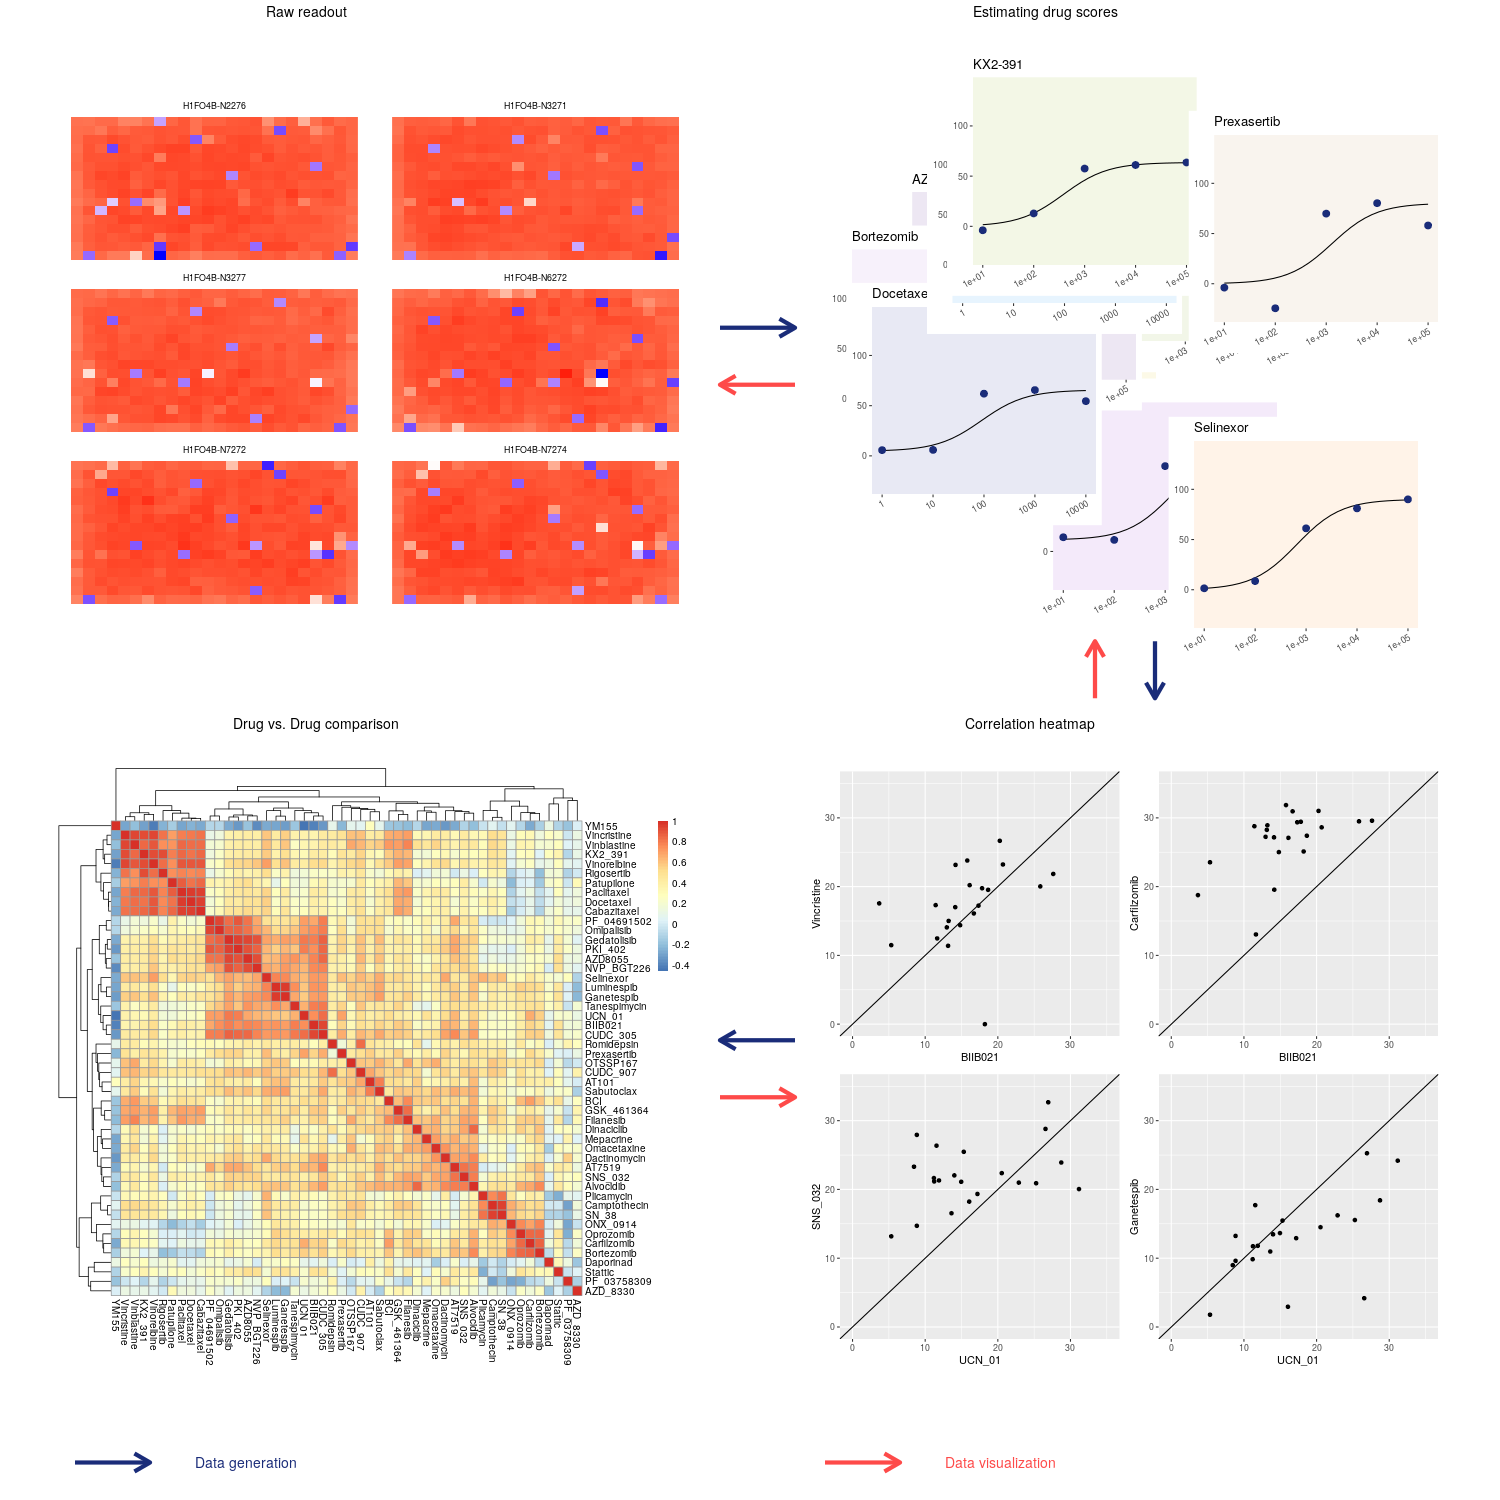
\includegraphics[width=\textwidth]{FigC/figC.png}
  \caption{The main idea behind the LinkedCharts library is shown based on a drug screening experiment. The blue arrow shows the direction of a typical pipeline used in drug screening experiments. We start with reading intensity values from plates with different cell lines grown in the presence of studied drugs (A). These values are then normalised and urned into a fraction of the cells that remained metabolically active (RealTime-Glo$^{TM}$ assay, \citep{rtg}) or maintain membrane integrity (CellTox$^{TM}$ assay, \citep{ctx}). A sigmoid curve is fitted to the obtained viability or toxicity values at different drug's concentrations, and the area under the fitted curve yields a single score for each drug (B). Different drugs' scores are compared to each other across all the tested cell lines (D). A drug-drug correlation heatmap is then produced to identify clusters of similar drugs (C). Red arrows illustrate the visualisation direction. We start by showing the summary heatmap plot (C). Suppose the researcher is interested in a particular drug combination or a cluster of drugs. In that case, he or she can examine the corresponding drug scores simply by clicking on the heatmap cell (D). Similarly, one can examine the exact viability values for any given drug (B). And finally, if needed, it is possible to take one more step back and to look at raw read-outs to inspect them for the presence of any artefacts (A).}
  \label{FigC}
\end{figure*}

To illustrate this idea, we can have a look at a typical drug screening pipeline based on data from \citet{he_2018}. In this study, a cohort of drugs was tested against pancreatic cancer cell lines and the value of interest was a score to measure drugs' efficiency. A pipeline was established to transform raw read-outs into more interpretable scores and then use them to explore drug profiles. Its flow is shown in Figure \ref{FigC} (there, only a subset of data is used for demonstration). The experiment starts from a cell viability assay on a microplate. The measured value is an intensity of fluorescence from each well that can be visualised as a heatmap with each cell representing a microplate well (Figure \ref{FigC}(A)). Then the raw values are normalised to obtain a percentage of metabolically active cells in each well. These values are now used to score each tested drug with the Drug Sensitivity Score (DSS, \citep{yadav_2014}). The score is based on the area under the sigmoid curve fitted to all five tested concentrations of the drug. Figure \ref{FigC}(B) shows some of these curves. Now there is a single value per drug-cell line combination. To find drugs with a similar efficiency profile, we can plot all the DSS values for each of the 21 tested cell lines against each other with two selected drugs as \emph{x} and \emph{y} axes (Figure \ref{FigC}(D)). Such a comparison produces a correlation value for each pair of drugs. Figure \ref{FigC}(C) shows them as a heatmap with clustered rows and columns, which allows one to study general patterns of drug groups with a similar effect on the cell lines. In Figure \ref{FigC} this flow of data generation is shown with the blue arrows.

To visualise the data with LinkedCharts, we should go backwards (red arrows in Figure \ref{FigC}). We start with the most generalised plot, which, in this case, is a correlation heatmap (Figure \ref{FigC}(C)). This is what a researcher would usually rely on to draw conclusions. However, one may want to manually check an interesting or suspicious pattern in the data before making any further claims. To this end, LinkedCharts allows to easily add another explanatory plot, that for each heatmap cell displays all the DSS values for the two corresponding drugs against each other (Figure \ref{FigC}(D)). A pair of drugs is selected by simply clicking on a heatmap cell. The drug score is also a summarised value that may be influenced by hidden artefacts in the data. If the researcher sees something out of place, he or she may want to check that as well. So we add another plot, showing the viability percentage for all five concentrations of the two selected drugs and the chosen cell line with the fitted sigmoid curve (Figure \ref{FigC}(B)). Just as the drugs are selected with mouse clicks on the heatmap, the cell line is picked by clicking on a point in the drug-drug plot. Finally, it is also possible to add the raw read-outs as the fourth plot (Figure \ref{FigC}(A)). In this example, it is linked to the drug-drug plot since all five concentrations reside on the same plate. But under other conditions, it can be linked to a viability plot and display the plate with the specific test.

Such a chain of charts where each one represents a major step of the data pipeline and is explained in detail by the next one is what R/LinkedCharts is particularly good at. These apps would allow a quick and easy spot check of uncovered data patterns and give the researcher a better understanding of inner connections between the data. For instance, to what extent noise can influence the signal or what is the scale of changes in the value of interest is typical to the data.

\subsubsection{Exploratory analysis}

While interactivity is already increasingly used to present results of finished studies to the research community, with R/LinkedCharts, we would like to point out its usefulness for everyday exploratory analysis. To this end, R/LinkedCharts is designed in a way that requires one to spend not more time designing an app than it would take to perform a similar analysis with static plots. One may think of R/LinkedCharts as a container where the researcher can put her or his code to turn it into an interactive app. It will not perform a complex analysis automatically, but it will also not ask for much more than the usual routine coding, one should do with or without interactivity. Basic yet custom and functional apps do not require any special knowledge of the package's underlying structure or HTML layout. With this, we have attempted to encourage researchers to try out interactivity as a more improvised and need-based approach.

Let us return to the example from Figure \ref{FigD}. There, we showed a typical part of a differential expression study: an MA plot (Figure \ref{FigD}(A)) and a plot with expression values for each sample to explore it (Figure \ref{FigD}(B)). We have already shown in Figure \ref{FigB} (Section ``Basic Syntax'') that making a static plot in R/LinkedCharts is not much different in comparison to popular plotting libraries. It will take the same effort and same data structuring and preprocessing to make these plots with, for example, the ``ggplot2'' library, as with ``rlc''. Now, the plot in Figure \ref{FigD}(B) serves for spot-checking. It allows one to dive into the details of expression patterns, but only for one gene at a time. Of course, one may decide to only rely on the general overview that is provided by the MA Plot (Figure \ref{FigD}(A)). However, a better practice is to make sure that there are no unexpected expression artefacts in the genes of interest. To do that, one would usually try to get a list of genes to check by filtering, using some special R tools, or somehow else, and then make a plot like the one in Figure \ref{FigD}(A) for each of them.

In the most simple case it would take copying and pasting the code for the spot check plot and replacing \mintinline{R}{y = normCounts["MyGene", ]} with \mintinline{R}{y = normCounts["AnotherMyGene", ]} (see the code chunk in Section ``Linking Charts''). A little improvement to that would be to write \mintinline{R}{y = normCounts[myGene, ]} and keep updating the \mintinline{R}{myGene} variable: \mintinline{R}{myGene <- "MyGene"}, then \mintinline{R}{myGene <- "AnotherMyGene"}. After each update one should still copy a piece of code that generates the plot into the console. Finally, the most effective way is to place this constantly copied and pasted code into a function, let say, \mintinline{R}{makePlot} and to call it, when necessary: \mintinline{R}{makePlot("MyGene")}, then \mintinline{R}{makePlot("AnotherMyGene")}.

Now, one can pause here and return to Section ``Linking Charts'', where the code to produce the app from Figure \ref{FigD} is given. The \mintinline{R}{onClick} function does the same thing that is described in the previous paragraph. It stores the new gene into the variable \mintinline{R}{k}. It then performs an equivalent of copying and pasting to the console the code for the second plot, which in the ``rlc'' library can be done with just the \mintinline{R}{updateCharts} function for the sake of simplicity. The core idea here is so identical to the usual spot-checking routine that one can add our imaginary \mintinline{R}{makePlot} function to the ``rlc'' chart, and it will still work. It is only essential to be aware that in this case, the argument to the \mintinline{R}{makePlot} will be an index of the selected gene and not its name.

Thus, there are simply no additional requirements to the data or environment, no new concepts that one should adopt to perform the usual exploratory analysis or even to convert an existing script into an interactive app. Figure \ref{FigE} shows such a transformation in details for another example of a common spot check practice.

\begin{figure*}[t]
  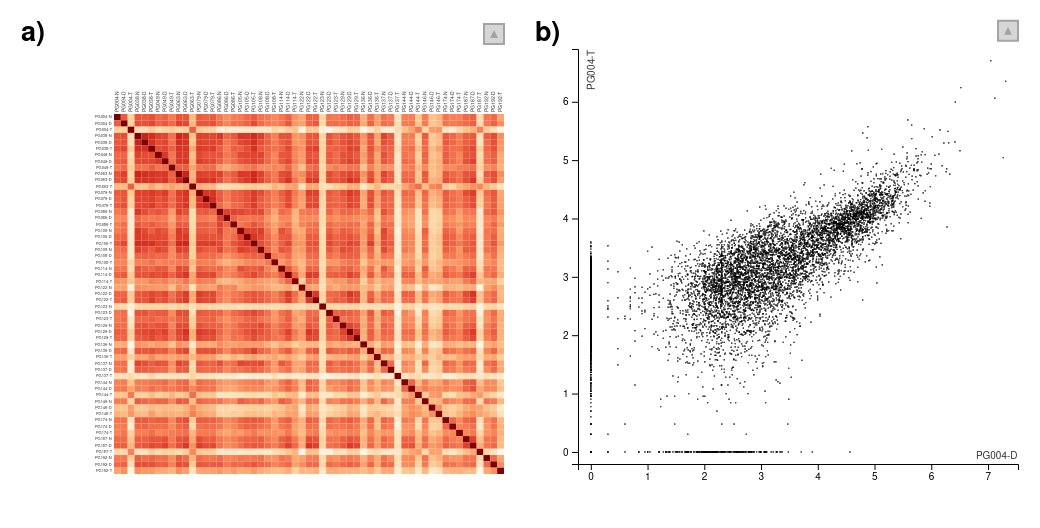
\includegraphics[width=\textwidth]{FigE/figE.png}
  \caption{ An example of an R/LinkedCharts app (C, D) that can be used during exploratory analysis and the code to generate it in comparison with the static plots (A, B) for the same purpose. The heatmaps (A, C) show Spearman correlation of gene expression for all samples from \citet{conway_2015}. Here, we can see two clear outliers in each heatmap's right and bottom and some more or less pronounced clusters of samples with similar gene expression levels. The scatter plots (B, D) show expression values for two samples plotted against each other. Browsing through several such plots can help the researcher get a feeling of the data and explore unexpected patterns like the outliers mentioned above. The code is split into two pieces, where the upper one is responsible for generating the plots and the lower part shows the code to update them. For static plots, one has to execute the same lines of code for any pair of samples he or she wants to compare, while for R/LinkedCharts the provided code should be added to the list of arguments for the heatmap. After that, switching between pairs of samples is done simply by clicking on the corresponding cell of the heatmap. The static heatmap (A) was generated with the ``pheatmap'' package  \citep{kolde_2019}; scatter plot (B) was made with a base R function. The live version of the app can be found in supplementary. For simplicity, gene expression for all the samples is subsetted to 8000 randomly selected genes.}
  \label{FigE}
\end{figure*}

This example is also based on the oral cancer data \citep{conway_2015}. Above, we have looked at differentially expressed genes between normal and cancerous tissues. Still, before getting there, a researcher who has just obtained these data may want to get some overview of the samples. e or she may want to check for the presence of batch effects, clusters or outliers. It is also useful to check whether the samples group together by origin or by type. One of the ways to do so is to have a look at a correlation heatmap. In Figure \ref{FigE}(A, C), for example, one can easily spot a small but tight cluster of samples and two outliers: the two samples to the right and bottom that are further from their nearest neighbours than most samples are from the majority of all others. The next most natural question to ask is how exactly these two samples are different from others. To answer it, one can plot gene expression values for several pairs of samples against each other (Figure \ref{FigE}(B, D)). It will give us a feeling of what ``similar'' means for the particular dataset and how the outliers do not fit this pattern. Therefore, the visualisation task at hand reminds the one described above and illustrated by Figure \ref{FigD}. Figure \ref{FigE} shows how to solve this problem with commonly used static plots (a heatmap from the ``pheatmap'' package \citep{kolde_2019} and a base R scatter plot, Figure \ref{FigE}(A,B)) and with R/LinkedCharts (Figure \ref{FigE}(C,D)). Below each set of charts, there is the code necessary to generate and update them. Neither the output nor the required commands are much different between the two. However, the R/LinkedCharts app is interactive. Besides linking, provides other useful features such as zooming in and out, reclustering heatmap and showing sample names when the mouse hovers above them.

This similarity makes R/LinkedCharts a helpful tool for exploration. The required effort to produce an interactive app is the same as to make traditional static plots. The only significant difference in the coding style that the user needs to get used to is to update one of the plots with a custom function and not by copying and pasting the same piece of code. However, such an approach is usually considered a better practice. In addition, the on-the-fly draft apps that were used for exploratory analysis can later be combined into a more complex app to present final results without a need to start from scratch.

\begin{figure*}[t]
   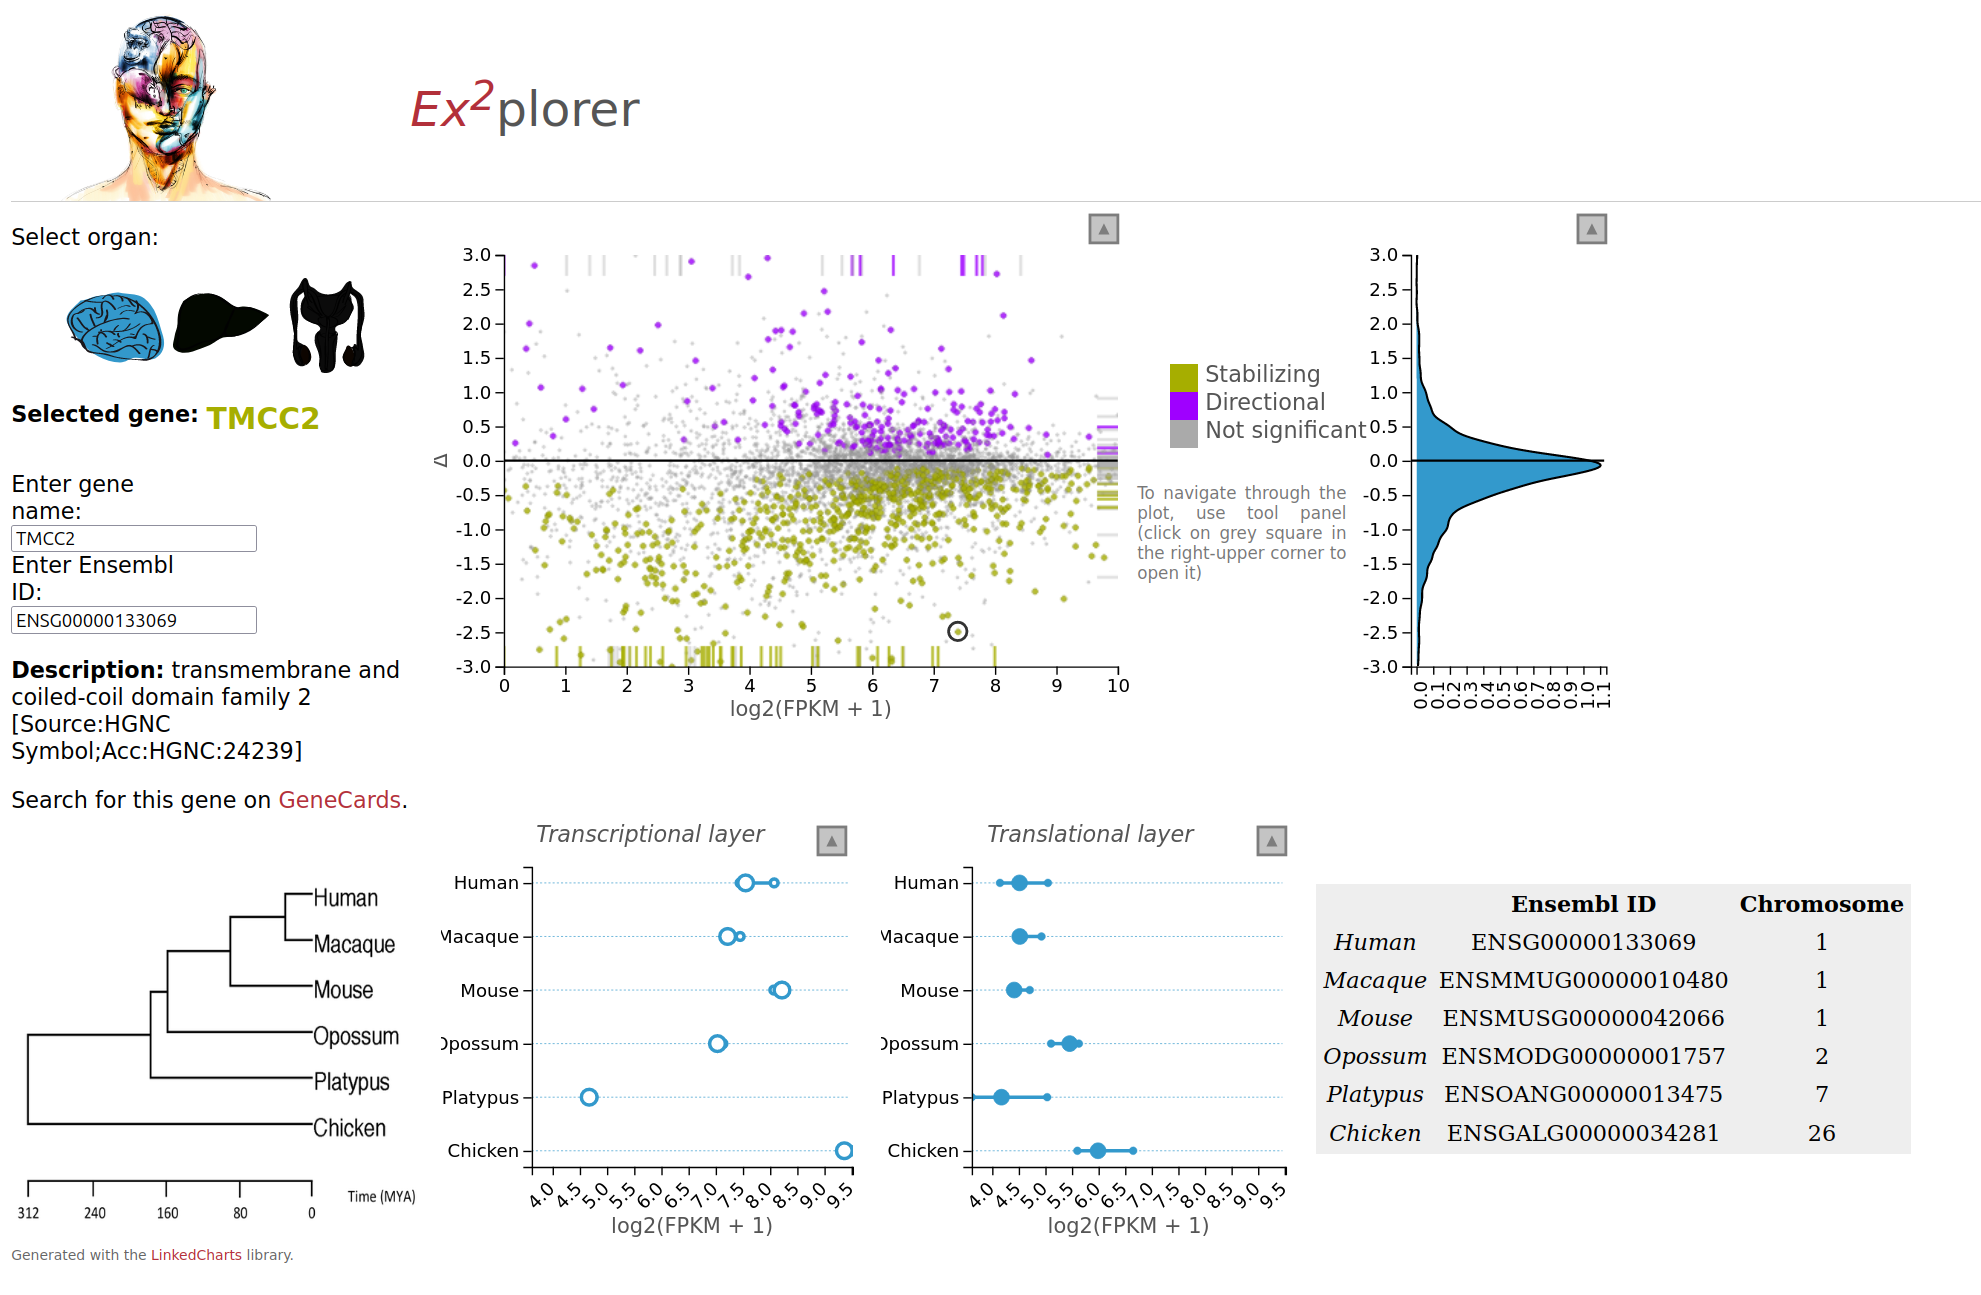
\includegraphics[width=\textwidth]{FigF/figF.png}
   \caption{An example of a stand-alone app with LinkedCharts. The app was used as a supplement for \cite{wang_2020}. Detailed information on the data, study goal and the source code for the app can be found in the related publication. The app is written in JavaScript and, thus, can be downloaded and opened in any modern browser without installation requirements. The app is based on the same principles as other examples throughout this paper. The main chart (upper row, centre) shows for every gene in the study its average expression and so-called $\Delta$-score, which indicates whether evolutionary changes in the translatome compensate for changes in the transcriptome or introduce new variance. The two plots below show expression values for the selected gene in all the tested samples. The user selects a gene by clicking on the corresponding point of the main plot or by entering the gene name (left upper corner). The density plot to the right shows the distribution of $\Delta$-scores, and its Y-axis is linked to the Y-axis of the main plot. In the upper right and bottom left corners, some additional information on the selected gene is displayed. Icons in the upper left corner allow switching between the studied tissues.}
   \label{FigF}
\end{figure*}

\subsubsection{Public apps}

All R/LinkedCharts apps start a server that listens to a given or randomly chosen port. To any request by a browser for the start page, this server answers with all the charts the user has added so far. In practice, it means that multiple users can access any R/LinkedCharts app if they can send a request to the server. Any of the examples we have shown in different sections of this paper can be made public by running them on a machine that can be accessed via the Internet. The code can be run without any changes or setting additional parameters, and already multiple users can access these apps, but their sessions will not be independent.

For the complete functionality, there is one more thing that has to be set. In a LinkedCharts app, one or several ``state'' variables are used. These are generally global variables that store currently selected genes, samples, etc. and are changed inside callback functions: \mintinline{R}{gene} from the example in Section ``Linking charts'', \mintinline{R}{xSample} and \mintinline{R}{ySample} from the example in Figure \ref{FigE}. If several users are working with these apps simultaneously, each click will change the state variables and consequently change the current state of charts for all the users. It can nevertheless be helpful if, for example, several people are using the app as a visual addition to an online meeting. Still, in most cases, one would like interactivity to be independent for each user.

To this end, is is only needed to enumerate state variables within the \mintinline{R}{openPage} function and give them some default values. For instance, the example from Figure \ref{FigE} can be turned into a public app simply by adding the following line in the beginning:

\begin{minted}{R}
openPage(sessionVars = list(
   xSample = 1, ySample = 2
))
\end{minted}

Now, multiple users can work with the app.

Of course, there are other settings to customise a public app. In addition to the charts, one can specify other default content for the page or scripts to be run for each new user. R/LinkedCharts provides tools to control each client session: for example, to close sessions inactive for specified time, limit memory usage or the number of simultaneously active connections. Still, all these parameters are optional. More information about possible options can be found on the R man pages for classes \mintinline{R}{App} and \mintinline{R}{Session} of our ``jrc'' package (available on CRAN).

\subsubsection{Stand-alone apps}

Any app made with R/LinkedCharts (``rlc'' package) requires a connection to a running R session. However, the R session is only responsible for sending the data to the app and updating them, while all the visualisation and interactivity handling happens on the JavaScript side. This fact makes it possible to use LinkedCharts for generating stand-alone apps in the form of an HTML page. Such a page can then be sent to a collaborator or used as a supplement file for a paper. Unlike a link to an app deployed somewhere on a server, this kind of interactive supplement will be available to any user with an installed web browser at any moment, without a need for the research team to maintain a running app on the server. A supplement to this paper is an example of such an app contained within an HTML page. Another app was made for \citet{wang_2020} and is published alongside it (\url{https://ex2plorer.kaessmannlab.org/}). A screenshot of this app is shown in Figure \ref{FigF}.

Such apps are possible since underneath ``rlc'' there is a fully functional and user-friendly JavaScript library \emph{linked-charts.js}. ``rlc'' simply offers a wrapper around \emph{linked-charts.js} and by means of the ``jrc'' package uses its JavaScript interface. Now, one can decide to do without the wrapper and use the \emph{linked-charts.js} library directly, and this is how stand-alone apps are made. Of course, they require some familiarity with JavaScript syntax and basic concepts. The extensive knowledge may only be necessary to perform complicated calculations directly in JavaScipt or define complex reactions to interactive events. ``rlc'' and \emph{linked-charts.js} are based on the same principles since one utilises the other. Because of this similarity, the conversion for simple apps is pretty straightforward. Every chart property turns from an argument of a plotting function into a method of the corresponding chart object. In most cases, neither property name nor input requirements changes, but callback functions to define property values are recommended for smoother interactivity. To get a feeling of these changes, one can look at the supplement to this paper. There, every example is provided together with R code and its equivalent in JavaScript.

The most complicated part of LinkedCharts stand-alone apps is loading the data. Due to security restrictions, JavaScript in a browser cannot access local files without the user explicitly uploading them. This makes data input quite tricky, despite a variety of existing parsers for most commonly used formats. The easiest way for an R user to solve this problem is to convert data into JSON format and directly insert it into the JavaScript code. JavaScript can then interpret the data as an array or an object. There are also other ways of loading data into a JS/LinkedCharts app, described in our tutorial \url{https://anders-biostat.github.io/linked-charts/js/tutorials/data.html}. Also, on this web page, one can find more tutorials and examples for a JavaScript part of the LinkedCharts library.

Unfortunately, we can not provide users with an automated converter of R/LinkendCharts apps into their JavaScript counterparts. Unrestricted customisation is an essential part of the ``rlc'' package. We want to provide researchers with a way to wrap any scientific ideas into an interactive app rather than fit the problem into a preset pattern. To this end, we do not limit users by a predefined set of callbacks, strict rules for data structuring or any other manipulations with the app. From a running R session, the user gets truly complete control over the app. Therefore, for reliable transformation of an ``rlc'' app into an HTML file, one needs a converter of R language to JavaScript, which, to our knowledge, does not exist.

Overall, one may find it complicated to get used to an unfamiliar language; however, I would like to conclude this section by pointing out the benefits of LinkedCharts stand-alone apps:

\begin{itemize}
   \item no R session needed;

   Not all hosting services allow to run R in the background, but a stand-alone app can be deployed almost everywhere. For instance, all the tutorials and examples mentioned in this thesis are hosted on GitHub Pages, a free and easy-to-use way to share one's project. In addition, stand-alone apps can be incorporated into an HTML presentation (made with \emph{reveal.js} or a similar framework).

   \item no server needed;

   In fact, a stand-alone app does not even need a server to be deployed since it can be downloaded by a user. A server generally requires some maintenance, renewed subscription, etc. Something may change over time that makes the app no longer accessible, and the research group may be no longer interested in keeping it running. A stand-alone app can be deposited together with the paper, and it will be available as long as the paper is. For example, check the supplement files for our paper \citep{ovchinnikova_2020}.

   \item an HTML file can be opened locally with any web browser.

   A stand-alone app is contained within a single HTML file (or several files for the sake of interpretability of the HTML code or to include figures). This file can be opened on any computer with a modern browser, and no other software installation is required. Thus, the app can be easily shared with collaborators from different areas of research who may be utterly unfamiliar with R.
\end{itemize}

\subsubsection{GUI apps}\label{gui_apps}

\begin{figure*}[t]
   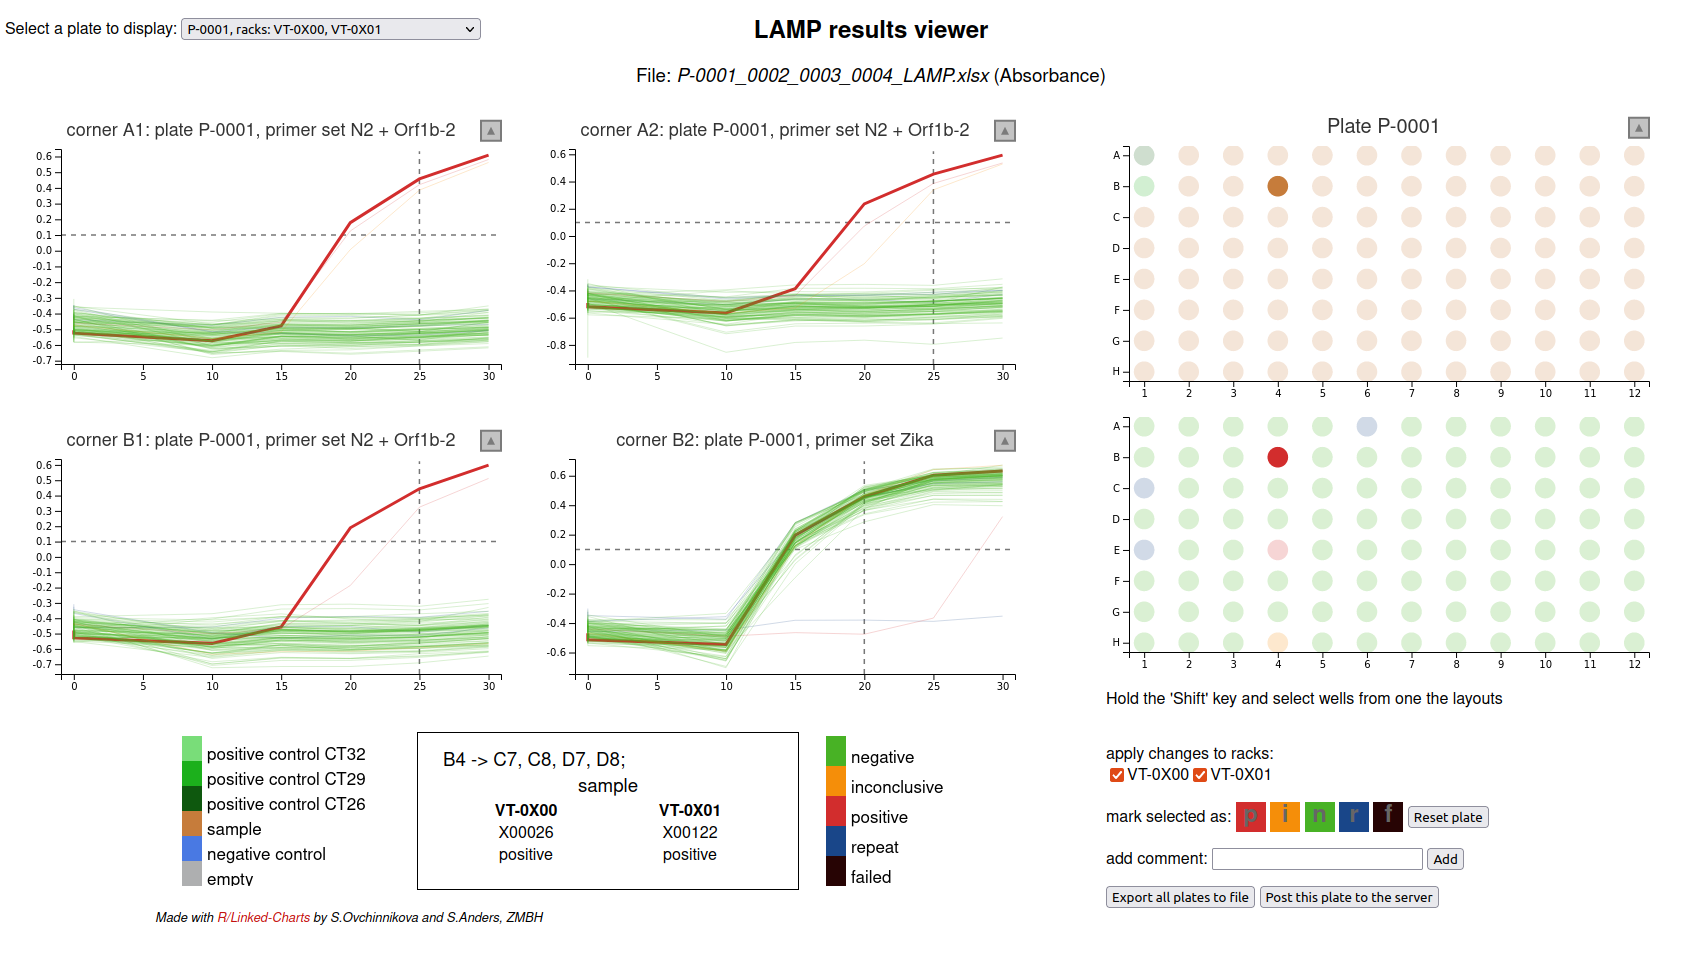
\includegraphics[width=\textwidth]{FigG/figG.png}
   \caption{An example of an app that was used as a GUI to perform manual inspection and classification of LAMP testing for SARS-CoV-19 viral RNA \citep{herbst_2021}. The app was used in the lab of Prof. Dr. Michael Knop (ZMBH) during the SARS-CoV-2 surveillance study \citep{deckert_2021} and for voluntary testing for Covid-19 infection on campus (University of Heidelberg) offered since June 2020. To the right, the app shows a 96-well plate layout coloured either by content type (sample, empty, positive or negative control) or by the assigned result. To the left, it shows the results of three tests and one control for each sample. Accumulation of the product is indicated by the change of colour from red to yellow and is measured as a difference in absorbance on two wave lengths. This difference is plotted as a function of time. Besides exploration (highlighting the corresponding lines for each sample), the app allows to manually reassign status, store results locally as a \emph{.csv} file or send them to the server, where they can be requested by people who provided the sample. The app is provided as an R script. It was used in-house and not published. However, the code and some example data are available on GitHub at \url{https://github.com/anders-biostat/lamp_plate_analysis}}.
   \label{lc_FigG}
\end{figure*}

Broad possibilities for customisation make it possible to use R/LinkedCharts for tasks beyond its primary goal (which is, as it follows from the name, linking several charts together for intuitive exploration). Since callback functions of the ``rlc'' package are not restricted to any predefined list of tasks, one can access the full spectrum of R functionality. Interaction with a chart cannot only update the app state but also store information in variables or external files, read new input from a file or ask the user for input, trigger some complicated calculations, send requests and data to a server. With all this, an R/LinkedCharts app can work as a graphical user interface for a custom R task.

To this end, the ``rlc'' package (\mintinline{R}{lc_input} function, see Figure \ref{FigA}G) offers a collection of elements to gather user input. The function provides a LinkedCharts interface to HTML ``input'' tag to add buttons, checkboxes, radio buttons, scrolls and text fields to the app. As any chart of the ``rlc'' package, the \mintinline{R}{lc_input} can get an R callback that is triggered every time the user changes the state of an input element (clicks a button or enters new text).

A screenshot of such a GUI app is shown in Figure \ref{lc_FigG}. The app is a part of the project dedicated to applying loop-mediated isothermal amplification (LAMP, \citep{notomi_2000}) for detecting SARS-CoV-2 virus \citep{herbst_2021}.

At the beginning of 2020, the advance of Covid-19 infection quickly led to the overloading of available testing capacities and, in turn, hindered prompt detection of the disease spread, especially by asymptomatic carriers. To address the issue, LAMP tests were offered at the University of Heidelberg as a cheaper and simpler alternative to commonly performed qPCR tests. Like PCR, LAMP allows detecting the presence of a specified DNA sequence in a saliva or swab sample, amplifying it with the help of pre-made primers. However, LAMP reaction does not require cyclic temperature changes and, thus, is much easier to perform. The disadvantage of this technique is that it is more stochastic than qPCR, and one may want to test each sample multiple times to increase accuracy. 

Within a few months, a pipeline for RT-LAMP tests for the presence of SARS-CoV-2 viral RNA in saliva samples was successfully established. In this pipeline, after RNA extraction, each sample was split to fill four wells of a microplate. Three wells were used for testing and one for positive control (with other primers that will lead to product accumulation in any sample). LAMP tests can be run as colourimetric or as fluorescent assays. In both cases, the plates were heated up to $65^\circ$C and changes in absorbance or fluorescence were measured periodically for the next 50 minutes. If the sample is positive, in about 20 minutes, it should change colour from red to yellow (which can be measured as a difference of absorbance on 560 nm and 437 nm wavelengths) or become fluorescent. Due to the stochastic nature of the LAMP reaction, the resulting curve of absorbance or fluorescence changes over time should be observed manually for reliable conclusions. And that is where interactive visualisation is most helpful.

After establishing the pipeline, the lab offered its testing capacity for students and employees on the campus of the University of Heidelberg who wanted to get tested for Covid-19 infection and, later, for randomly chosen participants of the SARS-CoV-2 surveillance study \citep{deckert_2021}. For their convenience, a website was created where people could register their samples and query the result. The interactive app from Figure \ref{lc_FigG} was designed as a mediator between the output of the plate reader and the web platform.

It served multiple purposes. First of all, it was used by the involved lab members to inspect the results of colourimetric or fluorescence RT-LAMP scans. This is important due to the stochastic nature of the LAMP reaction. The results of all four performed tests are displayed in the app as four sets of curves showing changes in absorbance or fluorescence over time. To the right, there is a 96-well plate layout used for RNA extraction, coloured by either the well content (sample, control, empty) or by the assigned status (positive, negative, inconclusive, failed). If the user hovers the mouse over a particular well, all four corresponding curves are highlighted (as it is shown in Figure \ref{lc_FigG}). And vice versa: hovering the mouse over any of the curves, highlights all other curves and the well for the corresponding sample. Thus, it was easy for the lab members to conclude the final status of the sample.

Another purpose of the app is manual classification. An automated classification is also performed as an initial step. However, in some cases, manual adjustments are required to account for some randomness in the reaction. In addition, a ``failed'' status, which means that the sample can not be tested at all, can only be set manually. Any sample can be selected to assign a new status by pressing a corresponding button in the right bottom corner. One can also add a comment to any sample. The results can be then stored as a \emph{.csv} file.

Finally, the third purpose of the app was to push all the results to the server, where they could be queried by people who have provided the samples. A new dialogue window then appears for the user to log in to the server, and then a report is generated both as a log file and as an information table.

The app was used during the SARS-CoV-2 surveillance study \citep{deckert_2021} and for free voluntary testing for Covid-19 infection offered on the campus of the Heidelberg University during the pandemic of 2020/2021. This app is made for in-house usage and tailored for the pipeline of the specific lab and, thus, is not published. However, the source code is available on GitHub at \url{https://github.com/anders-biostat/lamp_plate_analysis}. It is provided in the form of an R script that reads in and processes the output of the microplate reader and then uses it to add interactive charts to the pre-made HTML page. The page contains an empty layout and functions to populate and ensure the functionality of non-LinkedCharts interactive elements. The R script is also responsible for storing any changes that are made in the app, saving them as an external file and pushing the results to the server. All this functionality is defined either as charts' callbacks or independent functions called by the ``jrc'' package.

Overall, the app is an example of not only a GUI made with the ``rlc'' package but also how one can utilise the power of JavaScript and R for interactivity in combination with R/LinkedCharts to ensure the behaviour that perfectly fits the needs of the given project.

\subsection{Further customization}

Since LinkedCharts is JavaScript-based, it can be combined with many existing web solutions without changing the source code of the package. One can customise the charts' appearance with CSS, add additional scripts, specify an HTML layout. R/LinkedCharts can add interactive charts to an existing HTML page supplied as \mintinline{R}{startPage} argument of the \mintinline{R}{openPage}. Additional images, files or scripts can be loaded from a directory specified by the \mintinline{R}{rootDirectory} argument. In addition, more experienced users can take a step back and utilise the ``jrc'' package (available on CRAN) to employ the full power of JavaScript for reacting to user's actions. The ``rlc'' package is based on ``jrc'' and inherits its main classes and, therefore, full ``jrc'' functionality is available for any R/LinkedCharts app by default. All this gives the user full control of what the app looks like and how it functions. Therefore a LinkedCharts app can be fitted to the specific needs of the particular project.

\section{Discussion}

Interactivity has already proved itself to be useful for data visualisation. Static plots can accommodate only a limited number of accents. Any change, no matter how small, requires one to make a new plot. And yet, it is crucial to look at the data from different angles and on different scales to find peculiar patterns and make sure that there are no hidden artefacts that can influence conclusions. Sometimes, even the visualised transition from one state to another is what helps to understand the data. Thus interactive visualisation is helpful during the research and for presenting data to the scientific community.

The field of interactive visualisation is an actively developing one with some already well known and established tools such as ``shiny'' \citep{shiny} or ``plotly''\citep{sievert_2020}. Yet, possible benefits of interactivity are far from being explored. We have described LinkedCharts as a library for spontaneous and highly customisable visualisation. A simple interface makes R/LinkedCharts suitable for generating minor on-the-fly apps for data exploration. It can be used by researchers with only basic experience in R or by bioinformaticians who are not willing to invest much time into an acquaintance with an unfamiliar visualisation library. The linking mechanism is ensured by user-defined callback functions, allowing R/LinkedCharts to do without requirements for fixed data structures. There are no restrictions on the linking scheme. Every chart can be linked to any other or multiple ones. Any kind of backwards or partial linking is also possible.

We believe easy exploratory analysis to be the main niche for R/Linked charts. As we have shown, it provides users with a possibility to generate visualisations with the same effort as one generally puts into routine data digging and exploration. However, interactive apps are much more engaging than the static plots commonly used in the early stages of any project. When checking an idea or concern takes just a click, the researcher is more likely to go through the data thoroughly and, with this, maybe, save time on the further steps of the analysis.

Once the need to present final or intermediate results to colleagues arises, the same essential apps that were previously used as ``quick and dirty'' solutions can be prettified and shared by deploying the app on a server. The required changes for a R/LinkedCharts app to work on the server are minimal, and therefore there is no need to start from scratch. One can utilise the same scripts as personal drafts for exploration and as a basis for result presentation.

LinkedCharts is a JavaScript-based library, and unlike in existing alternatives, we gave users complete freedom to employ the functionality of various web solutions. For example, R/LinkedCharts can be embedded into any predefined HTML layout. Therefore, someone with experience in web design may provide the researcher with a custom HTML page with allocated containers for the chart and any predefined functionality made available by hundreds of JavaScript packages explicitly developed to ensure user interaction with a web page. Moreover, the ``jrc'' package on top of which R/LinkedCharts is built allows running any JavaScript code from the R session and any R code from the web page, providing endless possibilities for custom functionality and design. Such an app can also load locally stored scripts, images, stylesheets, etc.

The JavaScript basis of R/LinkedCharts offers an interface of its own that is also very simple and similar to the ``rlc'' syntax. Therefore a user who is familiar with JavaScript or willing to learn its essentials gets a way to convert R app into a stand-alone one fully contained within an HTML page. Such an app doesn't require any side resources, can be shared by email between collaborators and opened in any browser. It does not need to have a constantly running R session and can be published on any hosting, including the most simple ones that do not allow to run other software in the background. An example of such stand-alone apps is the supplement to this paper. There, one can also find examples of conversion from R apps to JavaScript ones. More information can be found in our online tutorials.

The structure of the JS/LinkedCharts library and even principles of JavaScript as a language to manipulate DOM elements can allow an experienced user to customise not just the ecosystem in which LinkedCharts will be embedded but the charts themselves without a need to dive into the source code. One can go as far as defining custom types of charts (see \url{https://anders-biostat.github.io/linked-charts/js/tutorials/layers.html} for more details on that).

Overall, R/LinkedCharts serves two primary purposes to facilitate data exploration and presentation. It offers an easy way to utilise interactivity for everyday research tasks. And it also provides the user with a possibility to fully employ the power of JavaScript for presenting the data. The latter aspect addresses more experienced users and thus has no limits for possible customisation of a LinkedCharts app.


\subsection{Implementation}

The JavaScript foundation of R/LinkedCharts is built on top of the D3 \citep{bostock_2011} library. JS/LinkedCharts is by itself a fully functional tool for interactive data visualisation that can be used by those familiar with JavaScript to create stand-alone apps. The library is open-source and available on GitHub at \url{https://github.com/anders-biostat/linked-charts}. The minified version can be downloaded from \url{https://github.com/anders-biostat/linked-charts/raw/master/lib/linked-charts.min.js}, and its stylesheet is at \url{https://github.com/anders-biostat/linked-charts/raw/master/lib/linked-charts.css}.

The ``jrc'' package \citep{jrc_2020} package is used as a bridge between R and JavaScript. It allows one to run JavaScript code from an R session and vice versa. It also is managing client connections to the app and is responsible for all the functionality necessary to deploy R/LinkedCharts apps on a server. ``jrc'' in turn is based mainly on ``httpuv'' \citep{cheng_2020} package to run a local server and ensure a WebSocket connection \citep{fette_rfc_2011}. 

R/LinkedCharts (``rlc'' package) is an R \citep{R_2019} interface to the JavaScript version of LinkedCharts. In addition to providing access to JS/LinkedCharts functionality, it also ensures proper storing of charts and serving them to each connected client by extending ``App'' class of the ``jrc'' package. ``rlc'' is open source and is available on CRAN or GitHub \url{https://github.com/anders-biostat/rlc}.

%\balance
\begin{small} 
\bibliography{lc}
\end{small}

\end{document}


